\documentclass{report}
%\usepackage[margin=5mm,a5paper]{geometry}

%Packages, die für die deutsch Sprache erforderlich sind
\usepackage[utf8]{inputenc}
\usepackage[T1]{fontenc}
\usepackage{lmodern}
\usepackage{ngerman}

%Packages für Graphik
\usepackage{graphicx}
\graphicspath{{Abbildungen/}}

%Optionen für Grafik
% Define new length
\newlength{\myFigureStandardWidth}
% Set the new length to a specific value
\setlength{\myFigureStandardWidth}{\textwidth}

%Package, damit Bibtex-URL klappt
\usepackage{url}

%Package für schöne Tabellen mit variabler Breite
\usepackage{tabularx}
\usepackage{booktabs}
\usepackage{multirow}

%Noch schönere Typographie (gibts nicht in Latexml)
%\usepackage{microtype}

%Pfeile für Chemische Formeln
\usepackage{amssymb}

%Package für Hyperlinks im PDF
\usepackage{hyperref}

%EBook-Package für die Titelseite
\usepackage{tex4ebook}

%Float-Placement
\usepackage{placeins}

\begin{document}
%%%%% BEGINN TITELSEITE %%%%%

\coverimage[width=1\textwidth]{Abbildungen/Titelseite.png} %TODO: Titelseite aktuell halten

%%%%% ENDE TITELSEITE %%%%%
\chapter*{Abstract}
\addcontentsline{toc}{chapter}{Abstract}
\section*{English}
\selectlanguage{english}
The behavior of several combinations of charging system and is calculated on two different bus lines using a simulation model. The input values for the simulation are the mechanical and electrical parameters of each charging system and battery, the mechanical parameters of the bus as well as a recording of one tour on the respective bus line. The simulation calculates the smallest possible battery to operate this bus line under user-definable constraints (e.g. overnight or opportunity charging), for each combination of battery and charging system. Battery size, energy consumption, battery cooling and charging time are calculated for each combination.

To assess the technological suitability of each combination, a weighted assessment according to VDI 2225 is performed on the simulation results. Significant differences in the suitability of different combinations were observed.

Using the method presented here transportation agencies and policy makers can obtain reliable data about the technological characteristics of different battery-driven buses in order to make an informed decision for a specific technology combination.

\section*{Deutsch}
\selectlanguage{ngerman}
Mit Hilfe eines Simulationsmodells werden technische Charakteristika von verschiedenen Kombinationen von Ladesystem und Speichertechnologien für zwei unterschiedliche Streckenführungen (Buslinien) berechnet. Eingangsdaten der Simulation sind mechanische und elektrische Parameter von verschiedenen Ladesystemen und Speichertechnologien, die mechanischen Parameter des Busses sowie die Aufzeichnung einer Linienverkehrs-Fahrt auf der jeweiligen Buslinie. Die Simulation berechnet für jede Kombination von Ladesystem und Speichertechnologie die kleinste Batterie, mit der diese Buslinie unter definierbaren Randbedingungen (z.B. Gelegenheits- oder Nachtladung) gefahren werden kann. Für jede Kombination werden Batteriegröße, Energieverbrauch, Batteriekühlung und Ladezeit berechnet.

Auf Basis der Simulationsergebnisse wird anschließend eine Bewertung nach VDI2225 durchgeführt, um die technische Eignung der verschiedenen Kombinationen zu vergleichen. Es zeigen sich deutliche Unterschiede in der Eignung verschiedener Technologiekombinationen.

Mit der in dieser Arbeit vorgestellten Methode können Verkehrsbetriebe sowie politische und wirtschaftliche Entscheidungsträger zuverlässige Daten über die technischen Charakteristika von verschiedenen batteriebetriebenen Bussen erhalten und auf dieser Grundlage eine fundierte Entscheidung für eine bestimmte Technologiekombination treffen.
\chapter*{Aufgabenstellung}
\addcontentsline{toc}{chapter}{Aufgabenstellung}

\tableofcontents
\newpage

%%%%% BEGINN INHALT %%%%%
\pagenumbering{arabic}

\chapter{Einleitung}
Die Klimaziele der Bundesregierung sehen eine Reduzierung der CO\textsubscript{2}-Emissionen im Verkehrssektor um 10\% bis 2020 und 40\% bis 2050 vor, jeweils gegenüber dem Niveau von 2005~\cite{BMUB-Referat-KI-I-1:2014}[S. 46]. Dafür soll der öffentliche Personenverkehr ausgebaut werden, da die Emissionen pro Passagierkilometer dort geringer als im Individualverkehr sind. Durch die Eliminierung fossiler Energiequellen können die verbleibenden CO\textsubscript{2}-Emissionen im öffentlichen Verkehr stark reduziert werden. Aufgrund der besseren Landausnutzung ist die Verwendung von Strom aus Wind-, Solar- und Wasserkraft attraktiver als der Einsatz von Biokraftstoffen in Verbrennungsmotoren.

Im Eisenbahnverkehr ist die direkte Stromversorgung aus Oberleitung oder Stromschiene eine erprobte und verbreitete Technologie. In Kombination mit erneuerbaren Energiequellen kann der CO\textsubscript{2}-neutrale Schienenverkehr also mit langjährig erprobten Technologien umgesetzt werden.

In Deutschland ist der Bus mit 34 Milliarden Passagierkilometern im Jahr 2012 nach Fern- und Regionalbahnen das drittstärkste öffentliche Verkehrsmittel~\cite{Verband-Deutscher-Verkehrsunternehmen:2013}[S. 13]. Der Stadtbus ist jedoch größtenteils auf Verbrennungsmotoren und erdölbasierte Kraftstoffe angewiesen. Oberleitungsbusse gibt es nur noch in wenigen Städten und ihre Wiedereinführung ist aus städtebaulichen Gründen nicht gewünscht. Um trotzdem sowohl CO\textsubscript{2}-Emissionen als auch Feinstaubemissionen zu minimieren wird aktuell in verschiedenen Projekten an Stadtbussen mit elektrischem Antrieb in Kombination mit Batterie- oder Wasserstoffspeicher geforscht. Diese Arbeit soll einen Beitrag zu dieser Forschung leisten.

\section{Geschichte}
\label{abs_geschichte}


Der batteriebetriebene Stadtbus ist eine Berliner Erfindung: Schon Ende Mai 1898 begann der Probebetrieb des ersten Elektrobusses~\cite{Risch:1957}. Dem in Abbildung \ref{abb_ersterEbus} gezeigten Elektrobus ist seine Abstammung von der Pferdekutsche noch klar anzusehen.  Im Jahr 1900 wurde der Prototyp im Linienbetrieb auf der Linie Anhalter Bahnhof – Stettiner Bahnhof (heute Nordbahnhof) eingesetzt. Aufgrund der geringen Zuverlässigkeit endete der Betrieb jedoch noch im gleichen Jahr. Ein Verwaltungsbericht des \emph{Königlichen Polizei-Präsidiums von Berlin – Abteilung Verkehrspolizei} fasste die Erfahrungen wie folgt zusammen:

\begin{figure}\centering
	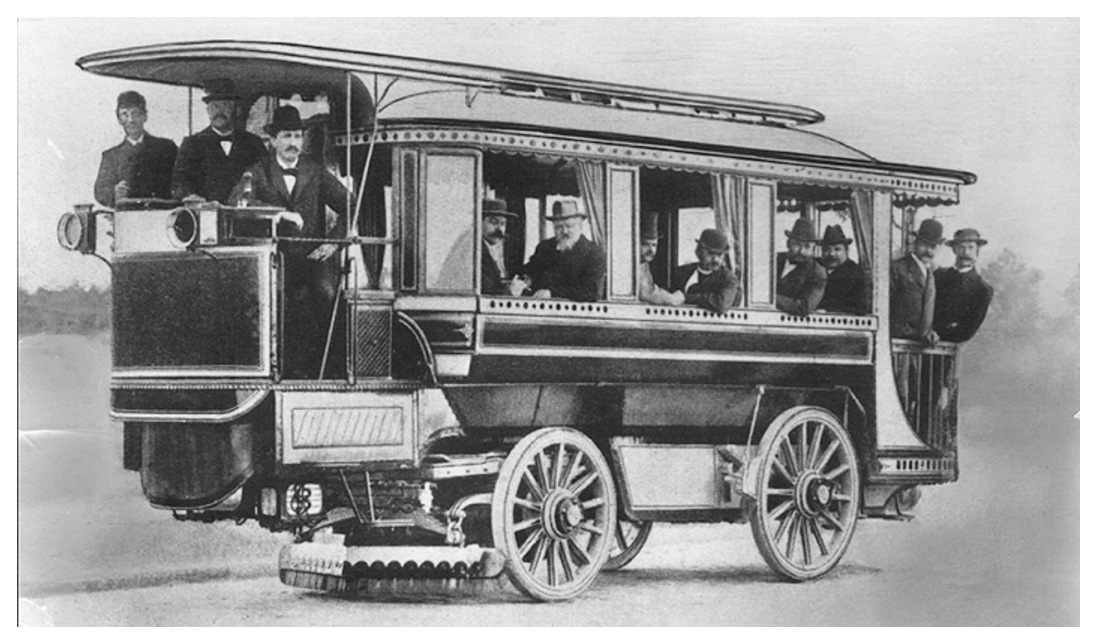
\includegraphics[width=\myFigureStandardWidth]{ersterEbus}
	\caption[Der Berliner Elektrobus 1898]{Der Berliner Elektrobus 1898. Quelle: \texttt{omnibusarchiv.de}}
	\label{abb_ersterEbus}
\end{figure}

\begin{quote}
	"`Das Urteil über die im Berliner Verkehrsleben bisher erschienenen elektrischen Omnibusse muß also dahin zusammengefaßt werden, daß dieselben zwar schon recht anerkennenswerte Leistungen auf dem Gebiete der elektrischen Fahrzeuge darstellen, jedoch von dem wünschenswerten Grade von Vollkommenheit noch ziemlich weit entfernt und bei dem jetzigen Stande der Technik zur Durchführung eines fahrplanmäßigen Omnibusbetriebes noch nicht geeignet sind."'~\cite{ersterEbus}
\end{quote}

Mit der Entwicklung zuverlässiger Verbrennungsmotoren rückte der batteriebetriebene Elektrobus für die nächsten Jahrzehnte in den Hintergrund. Der Einsatz von Bussen mit Schwungradspeichern in der Schweiz~\cite{tub_aleph001746639}[S. 216] und ein Testbetrieb mit Bleiakkus in einem Anhänger hinter dem Bus in Mönchengladbach~\cite{tub_aleph001746639}[S. 170] zeigten, dass die Speichertechnologie noch nicht ausgereift war. In den USA wurden in den neunziger Jahren Elektrobusse in Chattanooga eingesetzt, aber auch hier war der Einsatz auf kleine Busse und kurze Linien begrenzt~\cite{chattanoogaDOE}.

Mit der Entwicklung von preiswerten Lithium-Ionen-Akkus und Superkondensatoren nach der Jahrtausendwende können inzwischen auch große Busse und lange Buslinien elektrisch befahren werden. Parallel wurden leistungsfähige Ladetechnologien entwickelt, mit denen Busse nicht nur im Depot, sondern auch an End- oder Unterwegshaltestellen aufgeladen werden können.

\section{Der Berliner Elektrobus}
Im Jahr 2015 kehrt der Elektrobus nun nach 116 Jahren in den Berliner Linienverkehr zurück. Statt umgerüsteten Pferdekutschen und Bleibatterien werden nun Stadtbusse von Solaris und schnellladefähige Lithium-Titanat-Batterien verwendet. Der Bus ist in Abbildung \ref{abb_ebus2015} zu sehen. Die Berliner Verkehrsbetriebe (BVG) haben sich für ein induktives Schnellladesystem entschieden, mit dem die Busse an den Endhaltestellen in vier bis sieben Minuten aufgeladen werden können~\cite{ebus2015}. Die Technische Universität Berlin ist für die wissenschaftliche Begleitung dieses Projektes verantwortlich.

Die vorliegende Bachelorarbeit entstand im Rahmen dieser Begleitforschung des E-Bus-Projektes und im Zusammenhang mit dem Promotionsvorhaben von Tu-Anh Ly, dessen Ziel die Entwicklung einer methodischen und gesamtheitlichen Bewertung von Systemkonzepten für die Elektrifizierung von Stadtbussen ist.   

\begin{figure}\centering
	\includegraphics[width=\myFigureStandardWidth]{ebus2015}
	\caption[Der Berliner Elektrobus 2015]{Der Berliner Elektrobus 2015. Quelle: Oliver Lang / BVG}
	\label{abb_ebus2015}
\end{figure}

\section{Problemstellung der vorliegenden Arbeit}
\label{abs_problem}
Es existiert eine Vielzahl von Ladesystemen, Speichertechnologien und Ladestrategien. Der Bus kann konduktiv oder induktiv, manuell oder automatisch sowie bei Stillstand oder während der Fahrt aufgeladen werden. Es gibt viele verschiedene Batterietypen, die verschiedene chemische Reaktionen verwenden. Der Aufladevorgang kann über Nacht im Depot oder an den Endhaltestellen erfolgen. Die Vor- und Nachteile von verschiedenen Technologiekombinationen wirken sich bei unterschiedlichen Streckenführungen unterschiedlich aus. Von daher soll in dieser Arbeit die folgende Frage beantwortet werden:
\begin{quote}
	Welche Kombination von Ladesystem, Speichertechnologie und Ladestrategie ist für welche Buslinie am besten geeignet?
\end{quote}

\section{Methodik}
Um die in Abschnitt \ref{abs_problem} gestellte Frage beantworten zu können, werden zunächst detaillierte Daten zu den existierenden Ladesystemen und Speichertechnologien zusammengestellt. Es wird untersucht, welches Ladesystem für welche Ladestrategie geeignet ist und es werden Buslinien identifiziert, die als geeignete Beispiele für Modellrechnungen dienen können.

Um die Stärken und Schwächen einer Kombination von Ladesystem und Speichertechnologie auf einer bestimmten Buslinie beschreiben zu können, werden relevante Parameter wie Energieverbrauch, Masse, Ladezeit usw. mit einem Simulationsmodell berechnet.

Mit dieser Methode entsteht eine große Menge an Ergebnisdaten. Um diese Menge in aussagekräftige Ergebnisse umzuwandeln, werden die Ergebnisdaten nach systematischen Kriterien zusammengefasst und bewertet.
\chapter{Ladesysteme} %Zewitens
\section{Bewertungskriterien} %TODO: Subsections
% Mit welcher Methode ausgewählt?
\section{Betrachtete Systeme} %TODO: Subsections
\section{Vergleichstabelle}
\chapter{Speichertechnologien} %Zuerst
Nach den Ladesystemen sollen hier nun die Speichertechnologien betrachtet werden. Sie lassen sich in mechanische, elektrische und elektrochemische Speicher aufteilen. In diesem Kapitel werden die Wirkprinzipien der in Bussen verwendeten Speichertechnologien erklärt.\\
\section{Mechanisch – Schwungradspeicher} %TODO: Quellen, warum endete die Gyrobuserprobung
Mechanische Energiespeicher für Fahrzeuge arbeiten mit komprimierter Luft oder Schwungrädern. Es gibt Prototypen reiner Pressluftantrieben in kleineren Fahrzeugen, in Bussen werden sie jedoch nur als Teil eines Hybridantriebs eingesetzt und hier nicht weiter betrachtet.\cite{Sebastian-Naumann:2014}. Im Schwungradspeicher wird die elektrische Energie in der Rotationsenergie eines Schwungrades gespeichert, das sich mit sehr hoher Geschwindigkeit dreht. Die Energieübertragung erfolgt durch eine elektrische Motor- und Generatoreinheit. Moderne Schwungräder werden aus gewickelten Karbonfasern hergestellt und in Vakuumgehäusen magnetisch gelagert. Im Falle eines berstenden Schwungrades muss das Gehäuse die gesamte Energie innerhalb von Sekundenbruchteilen aufnehmen, ohne selbst zu bersten. Dies erfordert sehr schwere Gehäuse, die die spezifische Energie und Leistung eines tatsächlichen Systems stark reduzieren. Der Schwungradspeicher wurde in den fünfziger Jahren im Gyrobus im schweizerischen Yverdon auf einer acht Kilometer langen Linie erprobt. Die acht Kilometer lange Strecke wurde erfolgreich zurückgelegt, die damalige Technologie war jedoch sehr wartungsaufwändig. Aktuell wird der Schwungradspeicher nur als Teil eines hybriden Antriebsstrangs eingesetzt.
\section{Elektrisch – Kondensator} %TODO: Quellen
Der Kondensator ist ein rein elektrischer Energiespeicher. Im klassischen Plattenkondensator werden zwei durch ein Dieelektrikum getrennte Platten elektrisch aufgeladen und die Ladung kann später wieder in Strom umgewandelt werden. Kondensatoren haben eine hohe spezifische Leistung, aber ihre spezifische Energie reicht nicht aus. In Bussen werden sogenannte Superkondensatoren verwendet, die statt eines festen Dieelektrikums eine polare Flüssigkeit verwenden und mithilfe des sogenannten Doppelschichteffektes und der Pseudokapazität weit höhere Energiedichten erreichn. In Shanghai werden Busse mit dieser Technologie seit 2008 im Linienverkehr eingesetzt.
\section{Chemisch}
\cite{Lajunen20141}
\section{Bewertungskriterien} %TODO: Subsections
\section{Betrachtete Systeme} %TODO: Subsections
\section{Vergleichstabelle}   %TODO: In den Anhang?
\chapter{Effizienzberechnung} %TODO: Besserer Titel %Drittens
\section{Ladesystem}
\section{Speichertechnologie}
\section{Ladestrategie und Route}
\section{Ergebnisse}
\subsection{Route A}
\subsection{Route B}
\chapter{Bewertung und Diskussion} %Kapitelüberschriften
In den vorigen Kapiteln wurden technische Daten zu Ladesystemen, Speichersystemen und deren Kombinationen erhoben und berechnet. In diesem Kapitel wird nun eine gewichtete Bewertung dieser Kriterien erstellt, um Sinnhaftigkeit der verschiedenen Gesamtsysteme betrachten zu können.

Es muss darauf hingewiesen werden, dass die Systeme in dieser Arbeit aus rein technischer Sicht betrachtet werden und wirtschaftliche Aspekte ignoriert wurden. Von daher ist diese Bewertung nur im Zusammenhang mit einer Betrachtung aus wirtschaftlicher Sicht für Busbetreiber relevant. Systeme, die hier als technisch sinnlos identifiziert wurden können bei einer folgenden wirtschaftlichen Betrachtung ausgeblendet werden.

\section{Bewertungskriterien}
Die Auswahl und Gewichtung der Bewertungskriterien basiert auf der Masterarbeit von Thomas Pannwitz\marginpar{Formulierung, In QVZ als Dipl}, in der eine Umfrage unter 17 Busbetreibern über ihre Entscheidungskriterien für die Busbeschaffung durchgeführt wurde. Die fünf wichtigsten Anforderungen der Busbetreiber waren:
\begin{itemize}
	\item hohe technische Zuverlässigkeit des Fahrzeugs
	\item geringe Störanfälligkeit der Ladestation
	\item Verfügbarkeit von elektrischen Niederflurbussen
	\item Vermeidung von $CO_2$-Emissionen
	\item effizienter Einsatz unter extrem Umweltbedingungen\cite{pannwitz2014}[S. 24f]
\end{itemize}

Auf Basis dieser Kriterien wurde die in Tabelle \ref{tab_bewertungskriterien} dargestellte Zuordnung der technischen Daten zu den verschiedenen Kategoerien durchgeführt\marginpar{Gewichtung?}.



\begin{table}
	\centering
	\begin{tabularx}{\linewidth}{Xrl}
		\toprule
		Kriterium                        &                   & Gewichtung (\%) \\ \midrule
		\textbf{Reife}                   & $\Sigma$          & 25                    \\
		Fahrzeugkilometer, Teststrecke   &                   & 5                     \\
		Fahrzeugkilometer, Linienbetrieb &                   & 15                    \\
		Erfahrungen im Probebetrieb      &                   & 5                     \\ \midrule
		\textbf{Sicherheit}              & $\Sigma$          & 25                    \\
		Zugänglichkeit fahrzeugseitig    &                   & 10                    \\
		Zugänglichkeit stationsseitig    &                   & 15                    \\ \midrule
		\textbf{Komplexität Betrieb}     & $\Sigma$          & 25                    \\
		Freiheitsgrade gesamt            &                   & 5                     \\
		Positionierungsgenauigkeit       &                   & 10                    \\
		Kneelingfähigkeit                &                   & 5                     \\
		Anzahl der Wandler               &                   & 5                     \\ \midrule
		\textbf{Komplexität Aufbau}      & $\Sigma$          & 10                    \\
		Volumen im Fahrzeug              &                   & 5                     \\
		Aufwand für Bau der Ladestation  &                   & 5                     \\ \midrule
		\textbf{Effizienz}               & $\Sigma$          & 15                    \\
		Energieverbrauch                 &                   & 9                     \\
		Effizienz Energiespeicher        &                   & 2                     \\
		Effizient Ladesystem             &                   & 2                     \\
		Ladedauer pro Betriebsstunde     &                   & 2                     \\ \bottomrule
		                                 & $\Sigma_{gesamt}$ & 100
	\end{tabularx}
	\label{tab_bewertungskriterien}
	\caption{Gewichtung der Bewertungskriterien der Gesamtlösungen}
\end{table} 

%TODO : Am Anfang alles exakt, dann Vereinfachung mit hinweis darfauf, das exaktheit verloren

%TODO: Mehrere Tabellen, erst Rohdaten, dann mit Scorewerten, dann gewichteten

%TODO: Warum habe ich keine binäre Dominanzmatrix verwendet?


\section{Fazit}
\section{Ausblick}

%%%%% ENDE INHALT %%%%%

%Bibliographie
\bibliographystyle{alphadin}
\bibliography{../Quellen/Quellenliste} 

\appendix
\chapter{Datenblätter der untersuchten Energiespeicher}
\label{an_Datenblaetter}
\begin{figure}[h!]\centering
	%TODO: Kriege ich das Datenblatt
	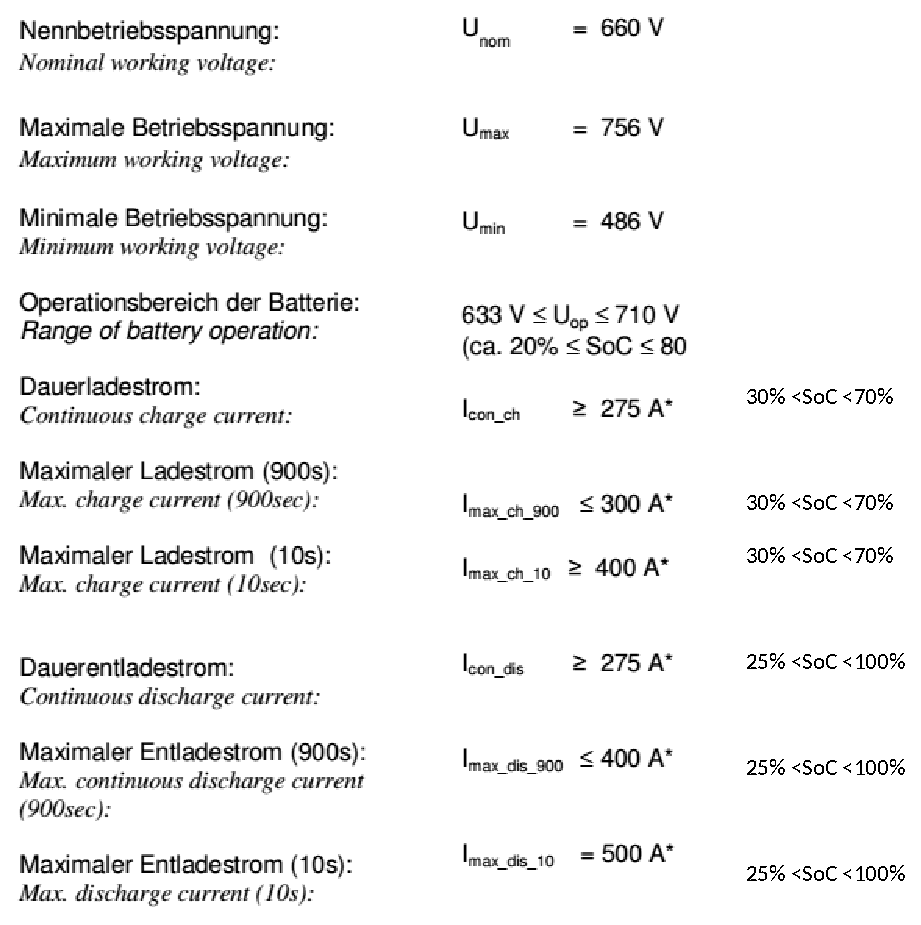
\includegraphics[width=\textwidth,height=0.8\textheight,keepaspectratio]{Datenblatt_LTO}
	\caption[Daten zum Primove-Akku]{Daten zum Primove-Akku. Quelle: MPM TU Berlin}
	\label{datasheet_LTO}
\end{figure}

\begin{figure}\centering
	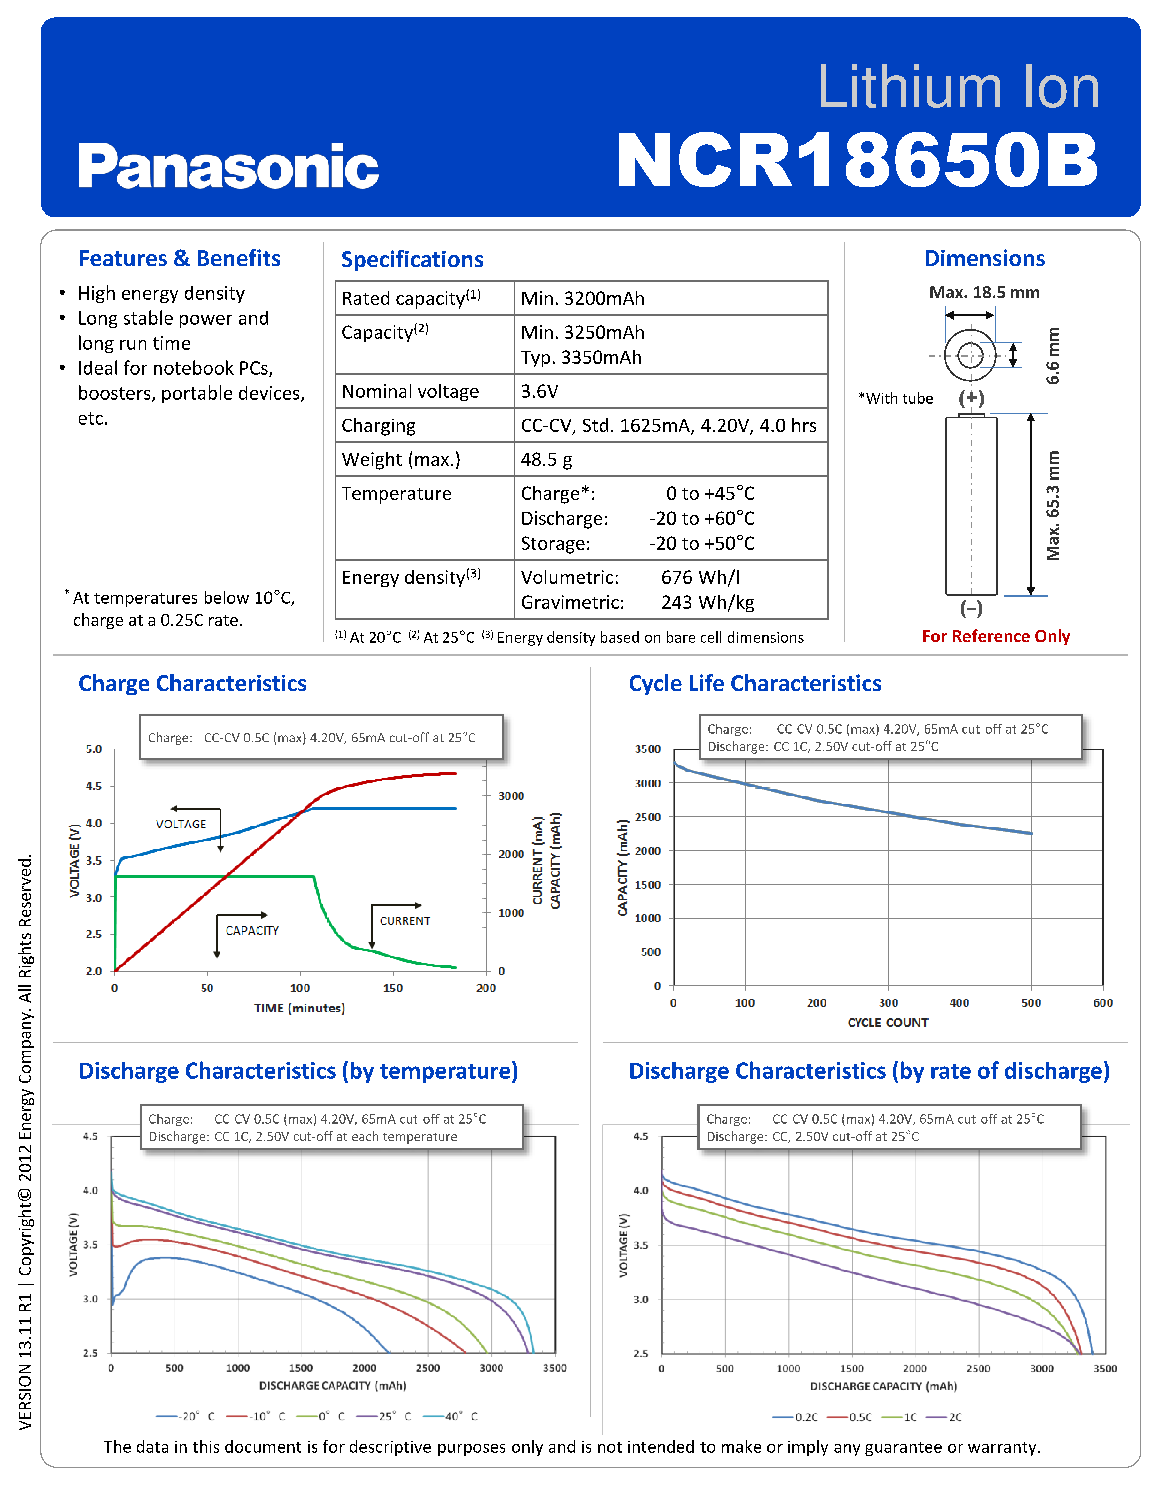
\includegraphics[width=\textwidth,height=\textheight,keepaspectratio]{Datenblatt_18650}
	\caption[Datenblatt Panasonic NCR18650B]{Datenblatt Panasonic NCR18650B. Quelle: Panasonic Industrial North America}
	\label{datasheet_18650}
\end{figure}

\begin{figure}\centering
	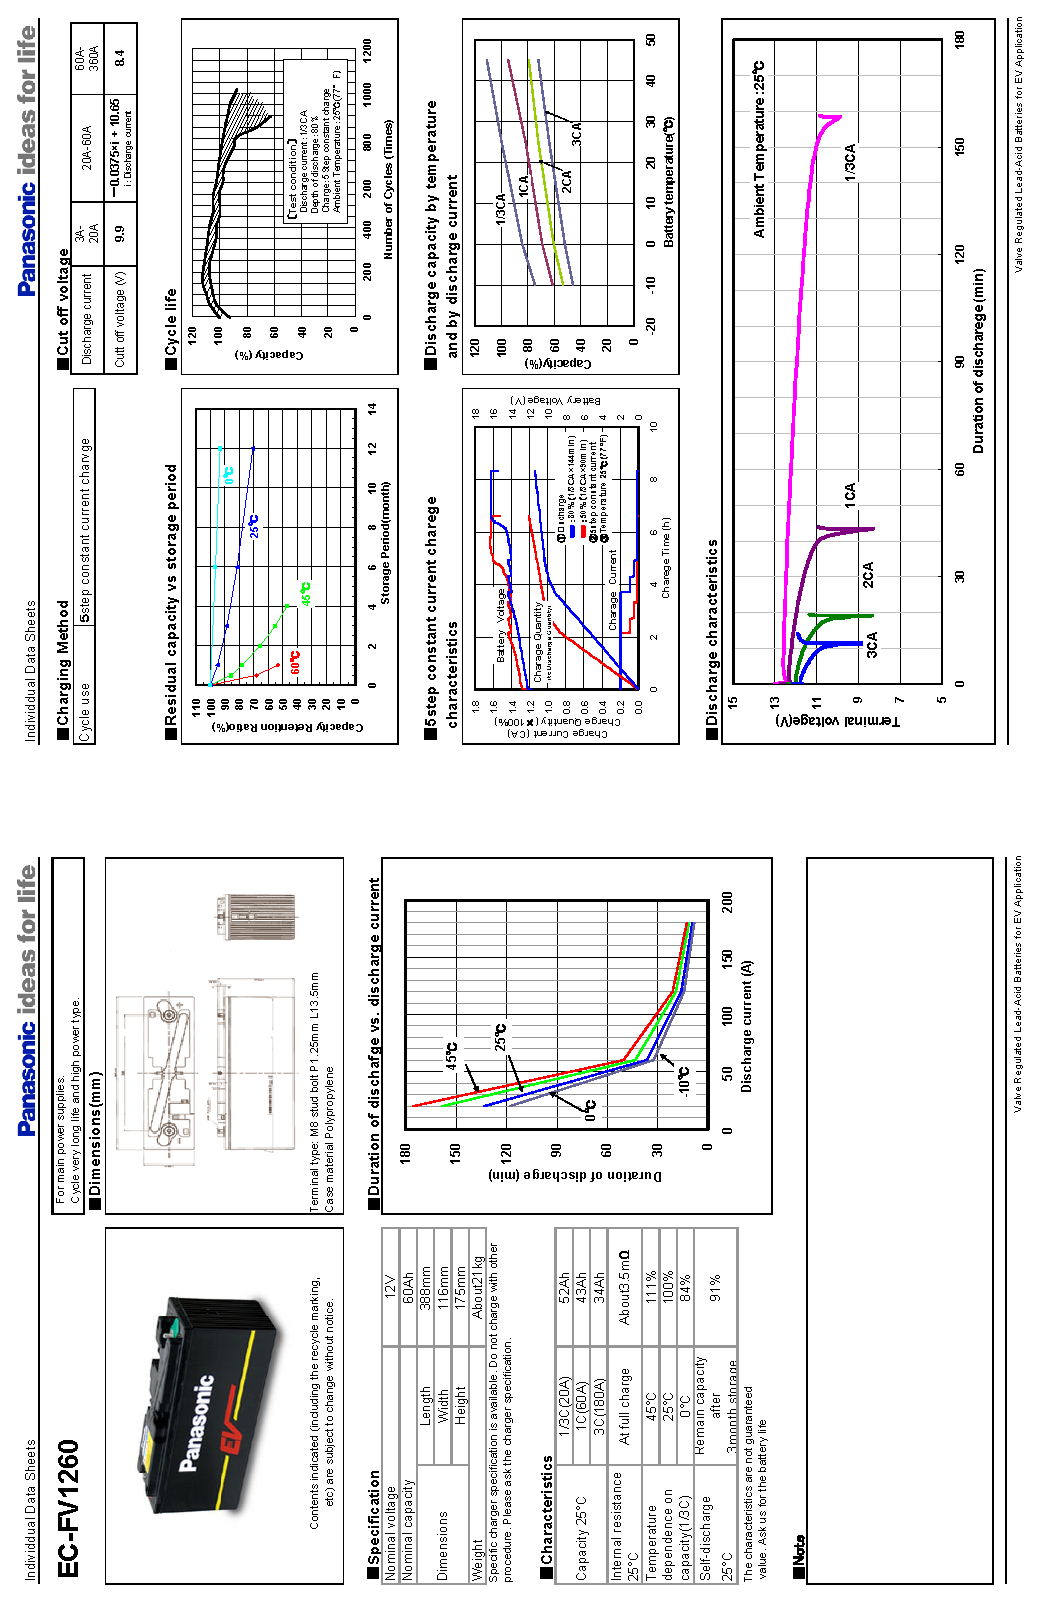
\includegraphics[width=\textwidth,height=\textheight,keepaspectratio]{Datenblatt_VRLA}
	\caption[Datenblatt Panasonic EC-FV1260]{Datenblatt Panasonic EC-FV1260. Quelle: Panasonic Industrial North America}
	\label{datasheet_Blei}
\end{figure}

\begin{figure}\centering
	\includegraphics[width=\textwidth,height=\textheight,keepaspectratio]{Datenblatt_LFP}
	\caption[Datenblatt European Batteries EV 45 Ah]{Datenblatt European Batteries EV 45 AH. Quelle: SuperLIB Deliverable 4.1 – Cell Specification with Cell Data}
	\label{datasheet_LFP_HE}
\end{figure}

\begin{figure}\centering
	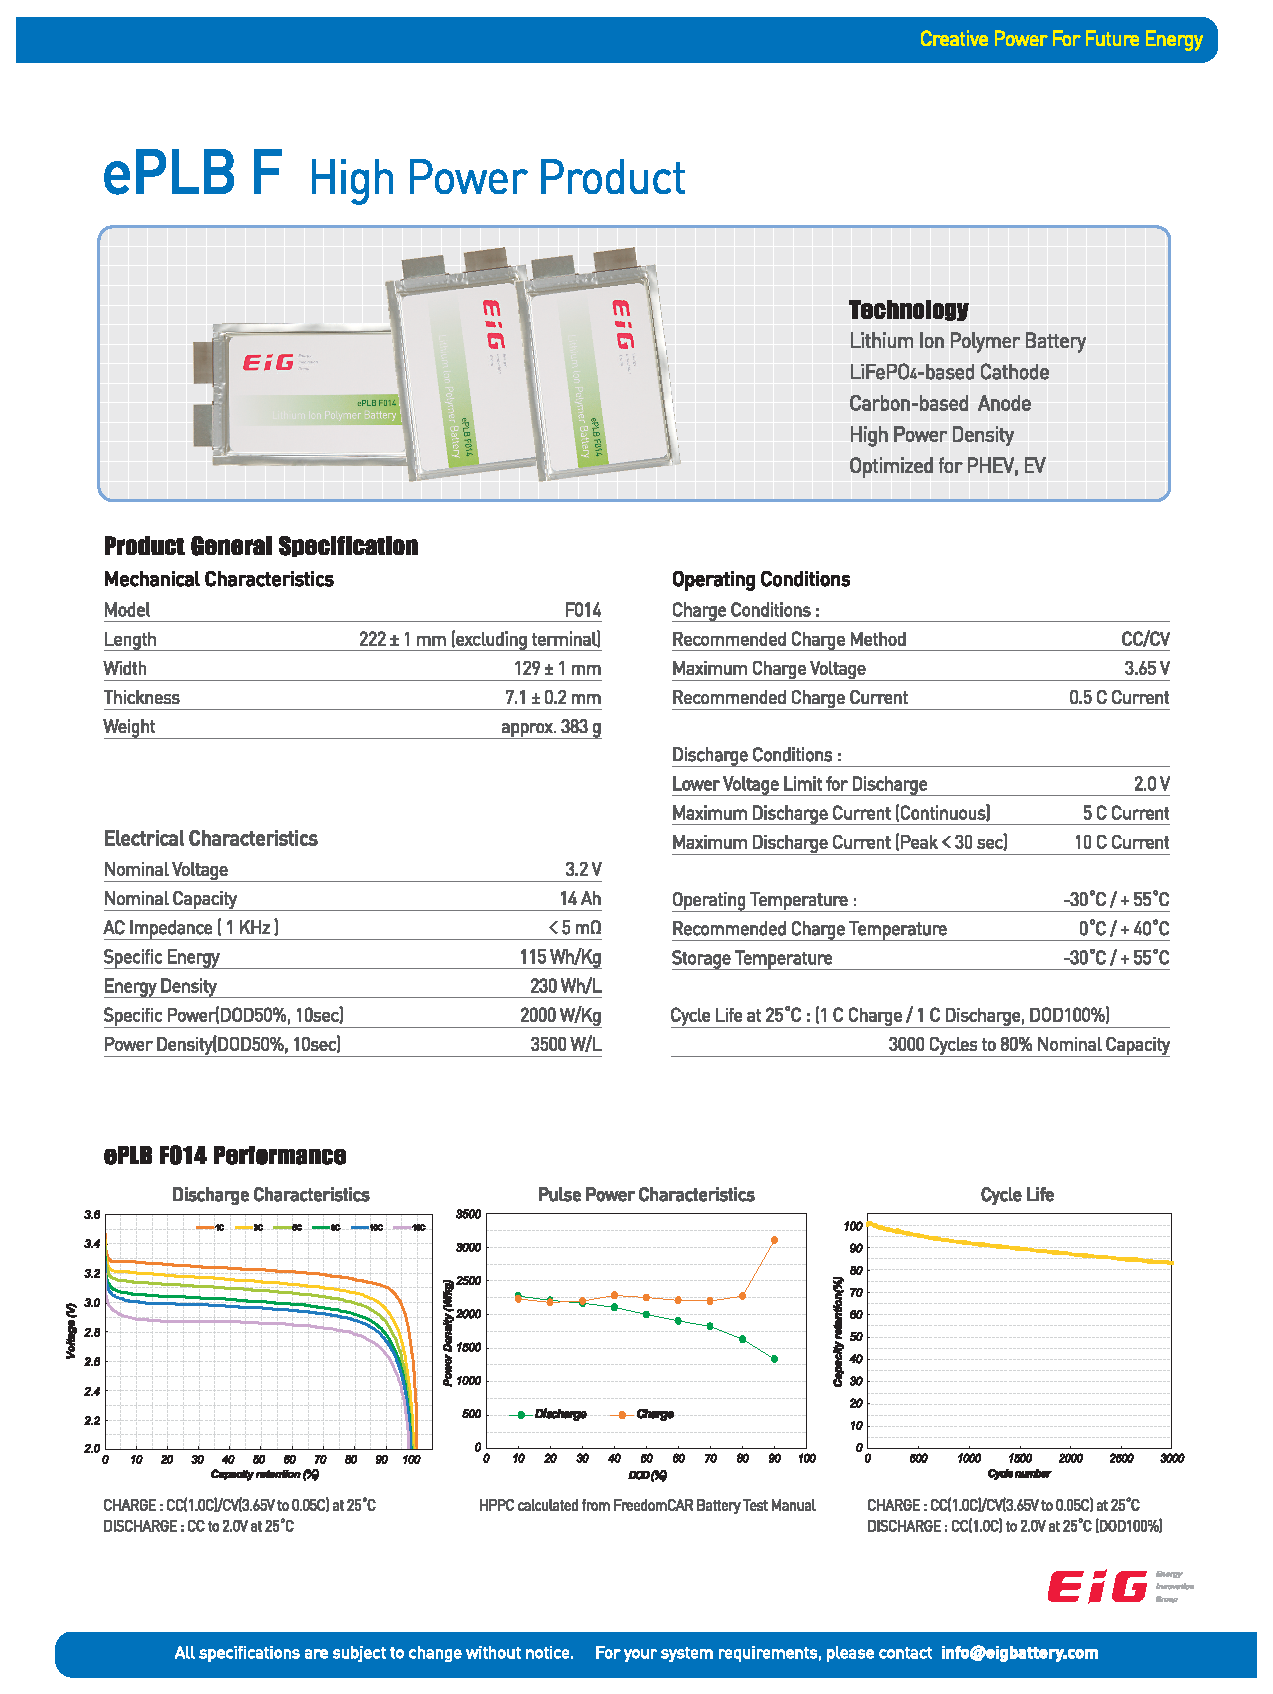
\includegraphics[width=\textwidth,height=\textheight,keepaspectratio]{Datenblatt_LFP_HP}
	\caption[Datenblatt EIG ePLB F 14 Ah]{Datenblatt EIG ePLB F 14Ah. Quelle: SuperLIB Deliverable 4.1 – Cell Specification with Cell Data}
	\label{datasheet_LFP_HP}
\end{figure}

\listoffigures
\listoftables

\end{document}
